\renewcommand{\chaptername}{}

\chapter{RESULTS}
 
This section will present the results of the experiments detailed in the Chapter 4 while providing 
some insight into what differentiates the fusion algorithms from the unimodal benchmarks. To do 
so, two different metrics are used to compare the algorithms. Average accuracy is the standard 
method for comparing classification algorithms. Since one of the goals of this paper is to improve 
the reliability of the overall system in diverse datasets, it is not beneficial to have near perfect 
accuracy for one class and sub-random choice on another class. This gap is smoothed out while 
comparing average accuracies, which is why these algorithms are reinterpreted as Montecarlo 
random algorithms. 

Montecarlo algorithms are randomized algorithms that have a deterministic runtime and a probability 
of returning the correct result. Random algorithms are generally measured in a worst-case scenario. 
So in this application the Montecarlo metric is defined as recognition accuracy for the worst class. 

Table 5.1 contains a summary of the accuracies of all the configurations. Each row represents an
 experiment, and it is summarized with the average of all the class accuracies, the standard deviation 
 of the class accuracies and the Montecarlo metric mentioned above.  The naming convention used
 to described each algorithm is as follows: 
 
 \[ \{\text{Method  AudioClassifier - LyricClassifier - MultimodalClassifier}\}  \]  
 
 Where Method can be a unimodal configurations (Audio or Lyrics) or a multimodal configuration 
 ( Full Ensemble, Audio Partial, Lyric Partial or Series ).
 
\begin{table}
\small{
	  \caption{Accuracy Measured in Average Accuracy and Montecarlo }
	\begin{tabular}{| c | l | c l  c  |  c|}\hline%
	& & Average & StdDev & Montecarlo\\\hline \csvreader[late after line=\\\hline]%
	{Averages.csv}{Algo=\name,Avg=\avg,Std=\std,Monte=\mte}%
	{\thecsvrow &  \name & \avg & \std & \mte}% 
	\end{tabular}
}
\end{table}
\newpage

It is interesting to notice some trends in Table 5.1. First note that overall accuracy for Fusion 
algorithms tend to be slightly higher than the accuracy for the unimodal benchmarks at the 
top of the table.  This is further explored by looking at the standard deviation of these 
accuracies; the benchmarks tend to have a higher variance the fusion experiments. This trend 
suggests that the audio only and the lyric only algorithms were very successful on a particular 
class while performing poorly on another one. Note that the Montecarlo metric tends to be higher
 when the standard deviation is lower.  Algorithms with a high Montecarlo value tend to do better
  overall.


Figure 5.1 contains a representation of all the benchmarks, which can be compared with Figure 5.2 
and Figure 5.3 that contain the two best fusion methods for each configuration. Figure 5.2 shows that 
Series methods do not perform very well. Looking at the other fusion methods, it becomes apparent that some preprocessing before fusing the data had drastic benefits.   Out of all the configurations with some preprocessing, 
Lyrics Partial Ensemble with SVM-Gaussian had the lowest overall accuracy of 62.8\% which is comparable
to the highest unimodal accuracy of 62.2\%.   Note that the majority of the Montecarlo values for 
the benchmarks are under 40\% while the Montecarlo value for all the fusion methods with preprocessing were over 55\%. 

\begin{figure}
\begin{minipage}[b]{\linewidth}
  \centering
  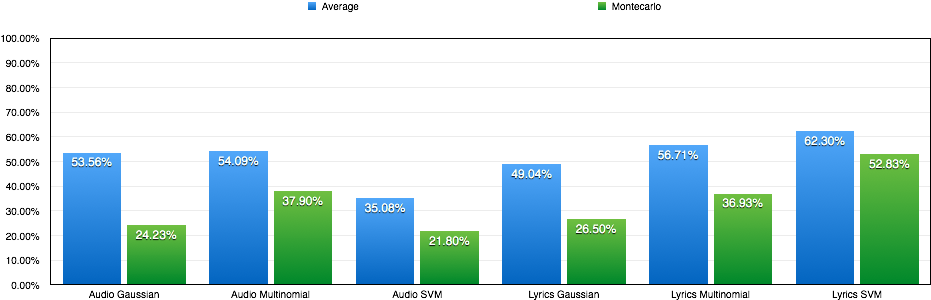
\includegraphics[width=1\textwidth]{Benchmarks.png}
  \caption{\small{Benchmark Summary}}
  \label{fig:blah1}
\end{minipage}
\hfill


\begin{minipage}[b]{0.6\linewidth}
  \centering
  \hspace*{-0.7in}
  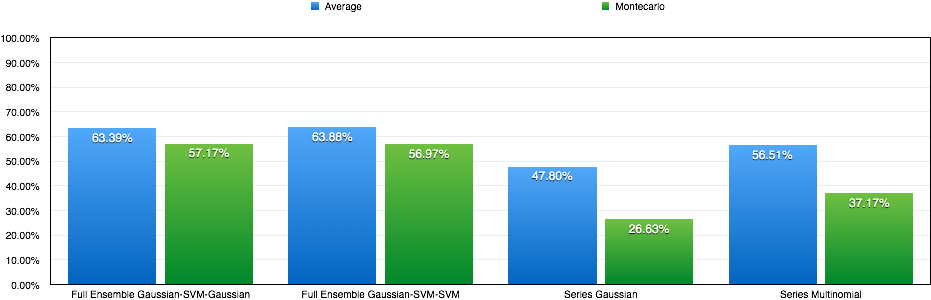
\includegraphics[width=1\textwidth]{EnsembleSeries.png}
  \caption{\small{Top of Full Ensemble and Series}}
  \label{fig:blah1}
\end{minipage}
\hfill
\begin{minipage}[b]{0.6\linewidth}
  \centering
      \hspace*{-.3in}
  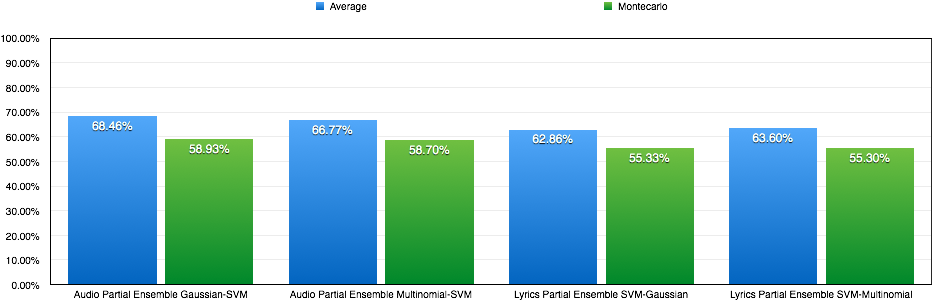
\includegraphics[width=1\textwidth]{Partial.png}
  \caption{\small{Top of each Partial Ensemble}}
  \label{fig:blah2}
\end{minipage}
\end{figure}

\section*{Better Reliability}

The Montecarlo value serves as an indication of how reliable the system is. 
A multi-class classification algorithm could possibly have strong average 
recognition accuracy as a result  of performing really well for one class but 
poorly for the others. Figure 5.4 shows the confusion matrices for the top 
two fusion algorithms and the top two benchmarks. The columns represent 
the true label "H", "S", "A" for the classes Happy, Sad and Angry. The rows 
represent the algorithm's prediction "h", "s", "a" for Happy, Sad and Angry.

Figure 5.4 is very informative in terms of what classes are harder to recognize. 
Clearly, happy songs are harder to identify that angry songs. This makes 
sense because angry words tend to only be present in angry music. For example 
words like "wrath" or "rage" are more indicative of emotion than words like "sunny" or "cheer".
 The same occurs with the Sad classification, but to a lesser extent. 

The benefit of the Montecarlo measurement becomes clear in Figure 5.4.d. 
This classifier has an average accuracy of 56.71\%, as seen in row 5 of 
Table 5.1. This classifier has some success for Sad and Angry classes, but 
makes a random guess for Happy songs.This type of behavior 
would be undesirable for a real application  

\begin{figure}
\centering 
\subfigure[Audio Partial Gaussian-SVM]{
		\begin{tabular}{l |c|c|c|}
			 & H & S & A\\
			\hline
			h & \textbf{58.93\%} & 15.60 \% &16.97\% \\
			\hline
			s & 19.93\% & \textbf{73.07 \%} & 9.67\% \\ 
			\hline
			a & 21.13\% &11.33 \% & \textbf{73.37\%} \\
			\hline
		\end{tabular}
	}
\subfigure[Audio Partial Mutimodal-SVM] {
	\begin{tabular}{l |c|c|c|}
	 & H & S & A\\
	\hline
	h & \textbf{58.70\%} & 19.00 \% &17.80\% \\
	\hline
	s & 18.70\% & \textbf{67.10 \%} & 7.70\% \\ 
	\hline
	a & 22.60\% &13.90 \% & \textbf{74.50} \\
	\hline
	\end{tabular}
}
\subfigure[Lyrics SVM]{
		\begin{tabular}{l |c|c|c|}
			 & H & S & A\\
			\hline
			h & \textbf{52.83\%} & 19.77 \% &17.27\% \\
			\hline
			s & 23.13\% & \textbf{63.93 \%} & 12.60\% \\ 
			\hline
			a & 24.03\% &16.30 \% & \textbf{70.13\%} \\
			\hline
		\end{tabular}
}
\subfigure[Lyrics Multinomial]{

	\begin{tabular}{ l |c|c|c|}
	 & H & S & A\\
	\hline
	h & \textbf{36.93\%} & 13.37 \% &7.87\% \\
	\hline
	s  & 32.23\% & \textbf{59.27 \%} & 18.20\% \\ 
	\hline
	a & 30.83\% &27.37 \% & \textbf{73.93} \\
	\hline
	\end{tabular}
}

\caption{Confusion Matrices for Top Fusion and Top Benchmarks}
\end{figure}

\newpage
\section*{Smaller Datasets}

Multimodal classifiers in general also tended to outperform unimodal 
classifiers on smaller training sets. Figure 5.5 shows the learning curves 
of the top fusion method and the benchmark using the Montecarlo 
metric. The training sets were compiled by taking 20, 50, 100, 500 
samples of each class. All the runs tested against a testing set containing 
100 samples of each class.  As seen in the figure, the multimodal classifier 
was consistently more reliable than the unimodal counterpart. For the 
smallest training set, Lyrics SVM  had an accuracy of 36.5\% which is barely
 above the random choice accuracy of 33\%. On the other hand, the Partial 
 Audio Gaussian-SVM classifier had an accuracy of 44.7\% on the smallest training set.
  It is clear that  even with very small datasets, multimodal outperforms unimodal classifiers. 

\begin{figure}
 \centering
 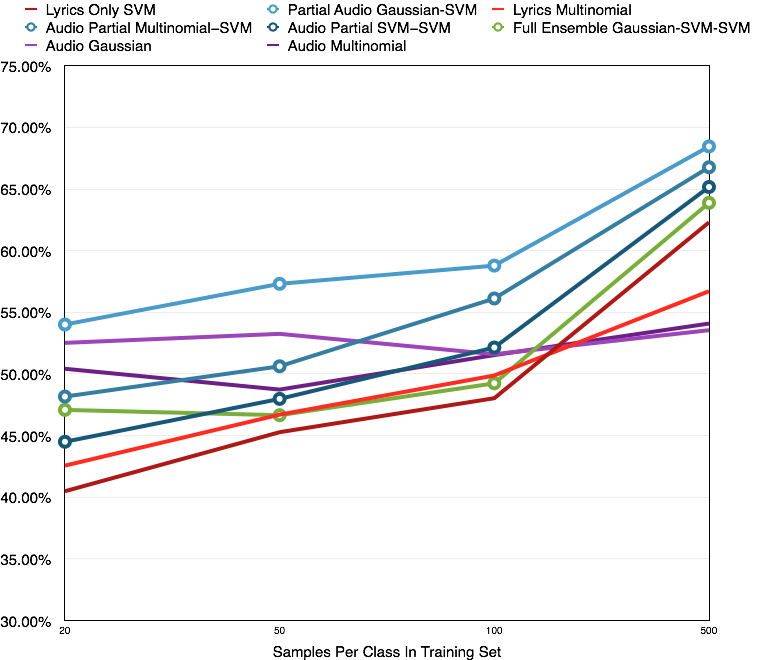
\includegraphics[width=\linewidth]{LearningCurves.png} 
 \caption{Learning Curves for Partial Audio Gaussian-SVM and Lyrics SVM}
\end{figure}


\chapter{FUTURE WORK}
This paper explored the benefits of combining classification methods in 
different configurations. It became apparent that the strongest configuration 
was the Partial Audio architecture with Gaussian preprocessing of Audio 
data and an SVM to classify the multimodal vector.  The features used for 
the paper were relatively simple to underline the added benefit of multimodal 
classification. Possible future work includes used more complex features that 
take into account sentence semantics to capture word modifiers. Another 
possible route for improvement on this paper would be to extend the number 
of classes used to all six Ekman emotions. 


